\documentclass[border=10pt]{standalone}
\usepackage{tikz}
\usetikzlibrary{arrows.meta}

\begin{document}
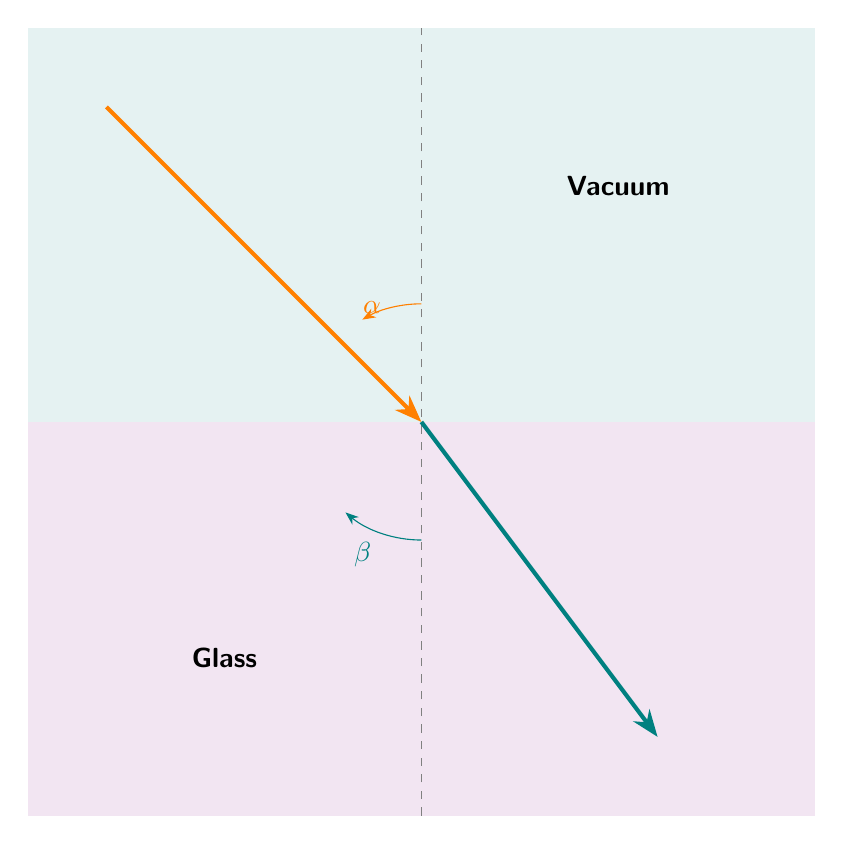
\begin{tikzpicture}[
    arrow/.style={-{Stealth}, line width=1.5pt},
    angle/.style={->, >=Stealth, orange},
    label/.style={font=\sffamily\bfseries}
]

% Background regions
\fill[teal!10] (-5,0) rectangle (5,5);
\fill[violet!10] (-5,-5) rectangle (5,0);

% Interface line
\draw[dashed, gray] (0,-5) -- (0,5);

% Light rays
\draw[orange, arrow] (-4,4) -- (0,0) node[midway, above left] {};
\draw[teal, arrow] (0,0) -- (3,-4) node[midway, below right] {};

% Angle alpha
\draw[angle] (0,1.5) arc(90:120:1.5) node[midway, left] {$\alpha$};

% Angle beta
\draw[teal, ->, >=Stealth] (0,-1.5) arc(270:230:1.5) node[midway, below left] {$\beta$};

% Labels
\node[label] at (2.5,3) {Vacuum};
\node[label] at (-2.5,-3) {Glass};

\end{tikzpicture}
\end{document}